The general second order equation can be expressed as follows,
\begin{align}
\vec{x^T}\vec{V}\vec{x}+2\vec{u^T}\vec{x}+f=0\label{eq:solutions/3/4/11/eq:1}
\end{align}
Comparing \eqref{eq:solutions/3/4/11/eq:0} with \eqref{eq:solutions/3/4/11/eq:1},
\begin{align}
\vec{V} = \myvec{5 & 1\\1 & 5}\label{eq:solutions/3/4/11/eq:2}\\
\vec{u} = \myvec{-7\\ -11}\label{eq:solutions/3/4/11/eq:3}\\
f = 27\label{eq:solutions/3/4/11/eq:4}
\end{align}
Let $\vec{c}$ be the change in the origin. The equation \eqref{eq:solutions/3/4/11/eq:1} can be modified as
\begin{align}
\vec{(x+c)^T}\vec{V}\vec{(x+c)}+2\vec{u^T}\vec{(x+c)}+f=0\label{eq:solutions/3/4/11/eq:5}
\end{align}
Considering \eqref{eq:solutions/3/4/11/eq:5}
\begin{align}
&\implies \vec{(x+c)^T}\vec{V}\vec{(x+c)}\\
&\implies \vec{x^T}\vec{V}\vec{x}+\vec{c^T}\vec{V}\vec{x}+\vec{x^T}\vec{V}\vec{c}+\vec{c^T}\vec{V}\vec{c}\label{eq:solutions/3/4/11/eq:6}
\end{align}
In the above equation
\begin{align}
\vec{c^T}\vec{V}\vec{x} = \vec{x^T}\vec{V}\vec{c}\label{eq:solutions/3/4/11/eq:7}
\end{align}
From \eqref{eq:solutions/3/4/11/eq:6} and \eqref{eq:solutions/3/4/11/eq:7} then \eqref{eq:solutions/3/4/11/eq:5} becomes
\begin{align}
\vec{x^T}\vec{V}\vec{x}+2\vec{c^T}\vec{V}\vec{x}+\vec{c^T}\vec{V}\vec{c}+2\vec{u^T}\vec{x}+2\vec{u^T}\vec{c}+f = 0\label{eq:solutions/3/4/11/eq:8}
\end{align}
Comparing \eqref{eq:solutions/3/4/11/eq:0.1} and \eqref{eq:solutions/3/4/11/eq:8}
\begin{align}
2\vec{c^T}\vec{V}\vec{P}\vec{y} + 2\vec{u^T}\vec{P}\vec{y} =0\\
\vec{c^T}\vec{V}\vec{P}\vec{y} = - \vec{u^T}\vec{P}\vec{y}\\
\vec{c} = -\vec{V^{-1}}\vec{u}\label{eq:solutions/3/4/11/eq:9}
\end{align}
Substituting \eqref{eq:solutions/3/4/11/eq:2} and \eqref{eq:solutions/3/4/11/eq:3} in \eqref{eq:solutions/3/4/11/eq:9}
\begin{align}
\vec{c}=\frac{-1}{24}\myvec{5&-1\\-1&5}\myvec{-7\\-11}=\myvec{1\\2 }\label{eq:solutions/3/4/11/eq:10}
\end{align}
Hence \eqref{eq:solutions/3/4/11/eq:8} becomes
\begin{align}
\vec{x^T}\vec{V}\vec{x}+\vec{c^T}\vec{V}\vec{c}+2\vec{u^T}\vec{c}+f = 0 \label{eq:solutions/3/4/11/eq:11}
\end{align}
Substituting \eqref{eq:solutions/3/4/11/eq:2}, \eqref{eq:solutions/3/4/11/eq:3} and \eqref{eq:solutions/3/4/11/eq:10} the above equation becomes
\begin{align}
\vec{x^T}\myvec{5&1\\1&5}\vec{x}+\myvec{1&2}\myvec{5&1\\1&5}\myvec{1\\2}+2\myvec{-7&-11}\myvec{1\\2}\\+27 = 0
\end{align}
\begin{align}
\vec{x^T}\myvec{5&1\\1&5}\vec{x}+29-58+27=0\\
\vec{x^T}\vec{V}\vec{x}-2 = 0\label{eq:solutions/3/4/11/eq:12}
\end{align}
With change in the origin to point $\vec{c}=\myvec{1\\2}$ but the $\vec{V}$ doesn't change.
\begin{align}
\mydet{\vec{V}} = \mydet{5&1\\1&5} = 24
\end{align}
As $\mydet{\vec{V}} >0$ it represents a ellipse.Hence $\vec{V}$ can be written as,
\begin{align}
\vec{V}=\vec{P}\vec{D}\vec{P^T}\label{eq:solutions/3/4/11/eq:13}
\end{align}
 The characteristic equation of $\vec{V}$ is given by
\begin{align}
\mydet{\vec{V}-\vec{I}\lambda} = 0\\
\mydet{5-\lambda & 1\\1& 5-\lambda} =0\\
\implies \lambda^2 - 10\lambda+24 = 0
\end{align}
Hence the eigen vales are,
\begin{align}
\lambda_1 = 4\\
\lambda_2 = 6
\end{align}
Hence diagonal vector is given by,
\begin{align}
\vec{D}= \myvec{\lambda_1&0\\0&\lambda_2} = \myvec{4&0\\0&6}\label{eq:solutions/3/4/11/eq:14}
\end{align}
The eigen vector $\vec{p}$ is given by
\begin{align}
    \vec{V}\vec{p}&=\lambda\vec{p}\\
    (\vec{V}-\lambda\vec{I})\vec{p}&=0
\end{align}
For $\lambda_1 = 4$  the eigenvector is,
\begin{align}
\vec{V}-\lambda_1\vec{I}= \myvec{1&1\\1&1} \xleftrightarrow[]{R_2 \leftarrow R_2-R_1}\myvec{1&1\\0&0}\\
\vec{p_1}=\myvec{\frac{1}{\sqrt{2}}\\\frac{-1}{\sqrt{2}}}
\end{align}
For $\lambda_1 = 6$  the eigenvector is,
\begin{align}
\vec{V}-\lambda_1\vec{I}= \myvec{-1&1\\1&-1} \xleftrightarrow[]{R_2 \leftarrow R_2+R_1}\myvec{-1&1\\0&0}\\
\vec{p_1}=\myvec{\frac{1}{\sqrt{2}}\\\frac{1}{\sqrt{2}}}
\end{align}
Hence,
\begin{align}
\vec{P} =\myvec{\vec{p_1}&\vec{p_2}} = \myvec{\frac{1}{\sqrt{2}}&\frac{1}{\sqrt{2}}\\\frac{-1}{\sqrt{2}}&\frac{1}{\sqrt{2}}} \label{eq:solutions/3/4/11/eq:15}
\end{align}
Substituting \eqref{eq:solutions/3/4/11/eq:14} and \eqref{eq:solutions/3/4/11/eq:15} in \eqref{eq:solutions/3/4/11/eq:13}
\begin{align}
\vec{V}= \myvec{\frac{1}{\sqrt{2}}&\frac{1}{\sqrt{2}}\\\frac{-1}{\sqrt{2}}&\frac{1}{\sqrt{2}}}\myvec{4&0\\0&6}\myvec{\frac{1}{\sqrt{2}}&\frac{-1}{\sqrt{2}}\\\frac{1}{\sqrt{2}}&\frac{1}{\sqrt{2}}}\label{eq:solutions/3/4/11/eq:16}
\end{align}
Hence substituting \eqref{eq:solutions/3/4/11/eq:16} in \eqref{eq:solutions/3/4/11/eq:12}
\begin{align}
\vec{x^T}\myvec{\frac{1}{\sqrt{2}}&\frac{1}{\sqrt{2}}\\\frac{-1}{\sqrt{2}}&\frac{1}{\sqrt{2}}}\myvec{4&0\\0&6}\myvec{\frac{1}{\sqrt{2}}&\frac{-1}{\sqrt{2}}\\\frac{1}{\sqrt{2}}&\frac{1}{\sqrt{2}}}\vec{x}=2\\
\vec{y^T}\myvec{4&0\\0&6}\vec{y}=2\\
\vec{y^T}\myvec{2&0\\0&3}\vec{y}=1\label{eq:solutions/3/4/11/eq:17}
\end{align}
where $\vec{y}$ is given by Affine transformation
\begin{align}
\vec{x}=\vec{P}\vec{y} \\
\vec{y}=\vec{P^T}\vec{x} \label{eq:solutions/3/4/11/eq:22}
\end{align}
The rotation matrix $\vec{P}$ can be given by,
\begin{align}
\vec{P}=\myvec{\cos{\theta}&\sin{\theta}\\-\sin{\theta}&\cos{\theta}}\label{eq:solutions/3/4/11/eq:18}
\end{align}
Comparing \eqref{eq:solutions/3/4/11/eq:15} and \eqref{eq:solutions/3/4/11/eq:18}
\begin{align}
\cos{\theta} = \frac{1}{\sqrt{2}}\\
\theta = \frac{\pi}{4} 
\end{align}
But given the direction of coordinate axes changes so,
\begin{align}
\theta = \pi +\frac{\pi}{4}\label{eq:solutions/3/4/11/eq:19}
\end{align}
Subtituting \eqref{eq:solutions/3/4/11/eq:19} in \eqref{eq:solutions/3/4/11/eq:18} we get 
\begin{align}
\vec{P}=\myvec{\cos{\brak{\pi +\frac{\pi}{4}}} & \sin{\brak{\pi +\frac{\pi}{4}}}\\-\sin{\brak{\pi +\frac{\pi}{4}}}&\cos{\brak{\pi +\frac{\pi}{4}}}}\\
\vec{P}=\myvec{\frac{-1}{\sqrt{2}}&\frac{-1}{\sqrt{2}}\\\frac{1}{\sqrt{2}}&\frac{-1}{\sqrt{2}}}\label{eq:solutions/3/4/11/eq:20}
\end{align}
From \eqref{eq:solutions/3/4/11/eq:13} we find the diagonal matrix
\begin{align}
\vec{D}=\vec{P^T}\vec{V}\vec{P} = \myvec{\frac{-1}{\sqrt{2}}&\frac{1}{\sqrt{2}}\\\frac{-1}{\sqrt{2}}&\frac{-1}{\sqrt{2}}}\myvec{5&1\\1&5}\myvec{\frac{-1}{\sqrt{2}}&\frac{-1}{\sqrt{2}}\\\frac{1}{\sqrt{2}}&\frac{-1}{\sqrt{2}}}\\
\vec{D}=\myvec{6&0\\0&4}\label{eq:solutions/3/4/11/eq:21}
\end{align}
Hence using \eqref{eq:solutions/3/4/11/eq:20}, \eqref{eq:solutions/3/4/11/eq:21} and \eqref{eq:solutions/3/4/11/eq:13} in \eqref{eq:solutions/3/4/11/eq:12} we get.
\begin{align}
\vec{x^T}\myvec{\frac{-1}{\sqrt{2}}&\frac{-1}{\sqrt{2}}\\\frac{1}{\sqrt{2}}&\frac{-1}{\sqrt{2}}}\myvec{6&0\\0&4}\myvec{\frac{-1}{\sqrt{2}}&\frac{1}{\sqrt{2}}\\\frac{-1}{\sqrt{2}}&\frac{-1}{\sqrt{2}}}\vec{x}=2
\end{align}
using \eqref{eq:solutions/3/4/11/eq:22} the above equation becomes,
\begin{align}
\vec{y^T}\myvec{6&0\\0&4}\vec{y}=2\\
\vec{y^T}\myvec{3&0\\0&2}\vec{y}=1\label{eq:solutions/3/4/11/eq:23}
\end{align} 
Hence from \eqref{eq:solutions/3/4/11/eq:17} and \eqref{eq:solutions/3/4/11/eq:23} proved that change of origin and the directions of the coordinate axes \eqref{eq:solutions/3/4/11/eq:0} can be tranformed to \eqref{eq:solutions/3/4/11/eq:0.1} or \eqref{eq:solutions/3/4/11/eq:0.2}
\begin{figure}[!ht]
\centering
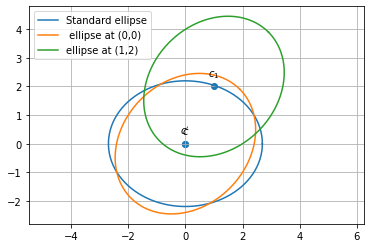
\includegraphics[width=\columnwidth]{./solutions/3/4/11/Ellipse.png}
\caption{Ellipse}
\label{eq:solutions/3/4/11/fig:Ellipse}
\end{figure}

